\chapter{Conceitos Básicos}
\label{cap:aspectos-basicos}

Nesse capítulo serão abordados os conceitos básicos utilizados neste trabalho visando a integração dos dados expostos na Internet. Em um primeiro momento, é realizado um estudo sobre o surgimento da Web Semântica e como as ontologias são utilizadas para agregar significado à informação visando à correlação dos dados. Abordam-se então as tecnologias e padronizações que auxiliam na propagação dessa proposta. Em um segundo momento, explora-se o contexto da Mineração de Dados, suas principais características, e como esta pode ser aplicada para auxiliar a evolução da Web Semântica. Por fim, verificam-se os diferentes modos de integração de dados e realiza-se uma síntese de tais técnicas, ilustrando como todos os conceitos abordados no capítulo podem ser aplicados de maneira a permitir a proposição de uma arquitetura voltada para a centralização de dados na Web capaz de permitir consultas mais ricas dentro de um determinado domínio de informação.

\section{Web Semântica}
\label{sec:Websemantica}

Atualmente a maior parcela dos dados disponibilizados na Internet é voltada para a leitura de humanos \citep{Berners-lee2001} e seu conteúdo é geralmente constituído por significados que não são compreendidos por máquinas. Além disso, nessa Web de dados os documentos estão interconectados por meio de âncoras de navegação, estruturas lógicas que apontam endereços da Web conhecidos por URLs (Uniform Resource Locator) que em conjunto formam uma grande infra-estrutura global. No entanto, dada a grande quantidade de informações exposta na rede se faz necessária a existência de um processo automatizado capaz de processar todo esse conteúdo disponível. Por esse motivo, tornou-se importante estabelecer maneiras que possibilitem às máquinas não só processar todo o dado disponível, mas também interpretar a informação assim como ela é compreendida pelos humanos. A Web Semântica é uma área de estudos que busca superar essa limitação de maneira a fazer não só com que a informação possa ser entendida pelas máquinas, mas também compartilhada e reutilizada na Web.

Para \cite{Berners-lee2001} a Web Semântica, ou simplesmente Web 3.0, é uma das mais importantes fontes de informação na Internet. É considerada uma extensão da Web Atual (Web 2.0) e não uma Web totalmente nova \citep{Yong-gui2010} uma vez que reutiliza os meios estruturais pré-existentes da informação, agregando-lhes uma camada de informação. Envolve um campo de pesquisa que tem por objetivo fazer com que os dados possam ser entendidos pelas máquinas \citep{Stumme2006} e busca promover meios para permitir uma infra-estrutura genérica capaz de realizar a integração de dados e incentivar o reúso de informação \citep{Bojars2008}. No entanto, a proposta central da Web Semântica não está em tornar a infra-estrutura da Internet atual mais inteligente, mas sim em utilizar formas de atribuir significado ao conteúdo dos documentos na Web a ponto de que a integração da informação entre eles não fique limitada apenas ao nível da camada de apresentação com os \emph{hyperlinks} \citep{Allemang2011}. 

A Web Semântica habilita as máquinas a compreenderem e manipularem de maneira mais eficiente os dados expostos na Internet. Isso decorre porque ao trazer suporte ao significado do conteúdo nos documentos, os computadores passam a trabalhar a informação de maneira mais próxima do que aquela que seria praticada por uma pessoa. A fonte de informação é similar àquela já utilizada na Web de hipertextos e baseia-se em documentos provenientes da Internet, mas diverge no que diz respeito à aplicação da semântica. Diferente da abordagem tradicional, no qual as ligações entre documentos são baseadas em âncoras de navegação que realizam o relacionamento em documentos HTML, na Web de dados é possível adicionar semântica aos sites a fim de construir uma ligação entre eles \citep{Bojars2008}. Desse modo, cada relacionamento entre entidades arbitrárias também pode ser descrito de maneira tal que uma pessoa ou máquina possa explorar a Web de dados; assim, ao ter acesso a uma pequena porção de informação, seria possível encontrar outros dados relacionados, formando uma teia de informações interligada, denominada Linked-Data. Nesta teia, todas as informações globais estão relacionadas e podem ser recuperadas a partir do mapeamento semântico com o uso de ontologias, de modo a tornar possível interligar dados diversos, como por exemplo bancos de dados mantidos por organizações geograficamente distribuídas \citep{Bizer2009}.

\subsection{Ontologias}
\label{sec:ontologias}

Ontologia é uma palavra que deriva do grego ``onto'' que significa ser e ``logia'' que representa o discurso escrito ou falado. É uma expressão cujas raízes estão situadas no campo da Filosofia a partir do estudo de teorias da natureza da existência \citep{Berners-lee2001}. Valendo-se desse contexto, os pesquisadores da Web de dados e da inteligência artificial passaram a adotar o termo para definir uma teia de conceitos, e relações entre eles,  de maneira que possam ser processados pelas máquinas. Desse modo, podem ser criadas taxonomias,  como apresentado na Figura \ref{fig:exemplo_taxonomia}, classificações, agrupamentos ou outras formas de representar domínios de conhecimento, geralmente visando o compartilhamento e reuso de dados.

\begin{figure}[!ht]
  \centering
  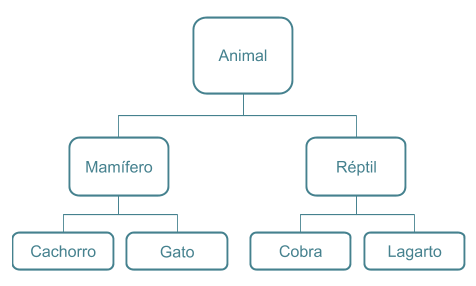
\includegraphics[width=.60\textwidth]{exemplo_taxonomia} 
  \caption{Exemplo de taxonomia}
  \label{fig:exemplo_taxonomia} 
\end{figure}

As ontologias são o coração da Web Semântica. São elas que formalizam o conhecimento sobre um domínio especifico de maneira a tornar possível a interpretação do significado de dados contidos em diferentes documento pelos computadores \citep{Bienvenu2013} permitindo dessa maneira um processamento automatizado e mais eficiente da informação. É freqüentemente definida como a especificação explícita de uma conceitualização \citep{Gruber1993} consistindo de diversos conceitos, expressos em uma linguagem que possui semântica bem definida, de fácil compreensão e leitura \citep{Gali2004, Kabir2014} e que dizem respeito a um contexto delimitado. Em outras palavras, trata-se da descrição formal explícita de conceitos que podem ser descritos como classes, formadas por atributos, e que descrevem características e restrições \citep{Jain2011}.

O problema da unificação de diferentes formas de dados pode ser superado por meio da exploração semântica com o uso de ontologias. Por serem caracterizadas por diversos conceitos a respeito de um domínio, acabam promovendo um entendimento único e compartilhado dos dados que existem dentro deste domínio. Desse modo, um dos objetivos mais comuns para o desenvolvimento de ontologias é o de compartilhar o entendimento comum da estrutura da informação \citep{Noy2001}. Assim, a Web semântica aproxima a possibilidade de realização de repositórios com dados organizados que podem ser utilizados para a pesquisa de informação inteligente para humanos e agentes computacionais \citep{Gali2004} na Internet. Regras de inferências nas ontologias adicionam ainda mais poder. Uma ontologia pode expressar uma regra para que um programa capaz de interpretá-la possa deduzir coisas como ``Se a Universidade de São Paulo está situada na cidade de São Paulo'' e ``São Paulo é uma cidade do Brasil'', então ``A Universidade de São Paulo está localizada no Brasil'' assim como representado na Figura \ref{fig:exemplo_inferencia}. Assim, as ontologias podem melhorar a funcionalidade da Web, aumentando a acurácia dos indexadores de informação e permitindo buscas mais ricas e sem ambigüidade acerca de um conceito.

\begin{figure}[!ht]
  \centering
  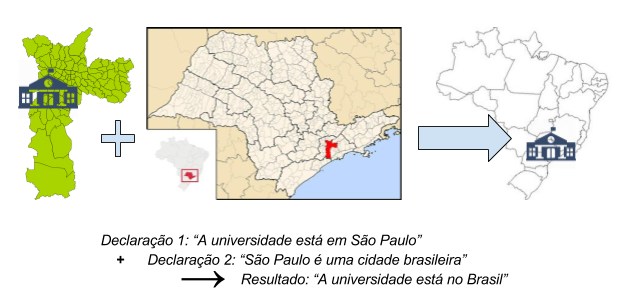
\includegraphics[width=.95\textwidth]{exemplo_inferencia} 
  \caption{Exemplo de inferência de regras}
  \label{fig:exemplo_inferencia} 
\end{figure}

\subsection{Exemplos de ontologias}
\label{sec:projetos_de_ontologias}

O crescente aumento no interesse da aplicação de ontologias para atribuição de significado aos dados incentivou estimulou a criação de projetos de padronização de conceitos. Essa normalização de significado busca alcançar um entendimento único e reaproveitável de conceitos a fim de  alcançar a integração dos dados expostos na Internet. Valendo-se desse contexto é que diversos esforços passaram a aparecer com maior força não só na comunidade cientifica mas inclusive na iniciativa privada.

Alguns dos projetos mais importantes nessa área são o \textbf{Schema.org} patrocinado pelos grandes indexadores de informação como Google e Bing, o vocabulário FOAF \citep{Brickley2010} (acrônimo Friend of a Friend) que busca descrever pessoas e relações e atividades entre elas, o DBPedia\footnote{\url{http://wiki.dbpedia.org/}} que busca elevar a informação da Wikipédia para a Web Semântica e o projeto Linking Open Data\footnote{\url{http://linkeddata.org/}} que pretende contribuir com o inter-relacionamento da informação na Internet a partir da aplicação de Web Semântica.

\subsubsection{Schema.org}
\label{sec:schema_org}
Interessados pela possibilidade de entregar conteúdo mais relevante e personalizado para seus usuários, os maiores portais de pesquisa de dados correntes, Google, Bing, Yahoo e o Yandex\footnote{\url{http://www.yandex.com/}} criaram a iniciativa Schema.org\footnote{\url{http://schema.org/}}. A idéia por trás desse esforço conjunto se traduz em melhorar a acurácia e apresentação de resultados da pesquisa nesses portais por meio da criação de marcações padronizadas que podem ser adicionadas pelos desenvolvedores das páginas HTML fazendo com que a máquina possa interpretar melhor os dados ali contidos \citep{Tort2014, Mika2015}. Desse modo, o portal Schema.org se estabeleceu com um conjunto padronizado de ontologias, constituído pela documentação dos conceitos e exemplos de uso das classes que representam os tipos de dados mais populares contidos na Web e construídas a partir de esforços já pré-existentes para a criação de terminologias, que estão sendo cada vez mais adotadas em larga escala \citep{Mika2015}. Entre os exemplos de definições contidas nesse repositório estão, por exemplo, o perfil de uma pessoa bem como as propriedades que o definem, informações sobre produtos, entidades de negócio, eventos, organizações, restaurantes, entre muitos outros. 

A Figura~\ref{fig:exemplo_organizacao_schema_org} ilustra o que seria uma organização do ponto de vista semântico e exemplifica como essas ontologias podem ser utilizadas em documentos na Internet. Nesse exemplo, podemos notar a descrição de uma organização (Organization\footnote{\url{http://1.schemaorgae.appspot.com/Organization}}), a quantidade de vezes em que ela foi utilizada em diferentes portais da Web, as propriedades que ela possui, i.e, endereço (\emph{"address"}), email, entre outros; além disto, descreve-se também o tipo de cada uma dessas propriedades, juntamente com uma breve descrição de cada uma delas.

\begin{figure}[!ht]
  \centering
  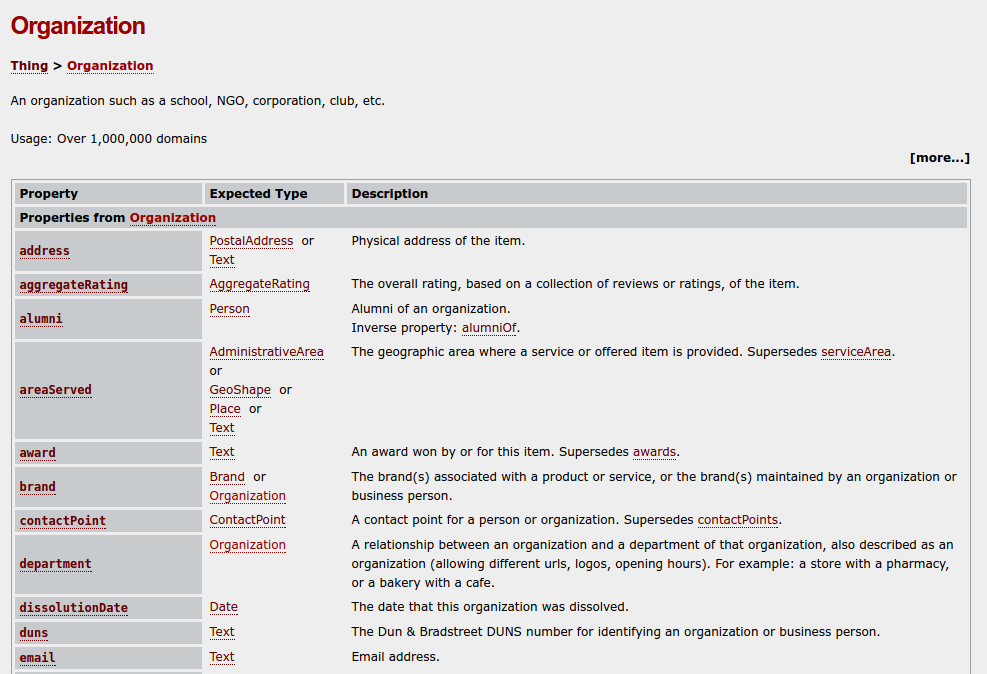
\includegraphics[width=.95\textwidth]{exemplo_organizacao_schema_org} 
  \caption{Exemplo da definição de uma organização pelo projeto Schema.org}
  \label{fig:exemplo_organizacao_schema_org} 
\end{figure}

\subsubsection{DBPedia}
A enciclopédia digital  Wikipédia\footnote{\url{https://www.wikipedia.org/}} é hoje um dos portais mais importantes do planeta, contando com informações nas mais diversas linguagens. Nele é disponibilizado o esforço de uma produção colaborativa de pessoas que produzem o conteúdo e que o revisam para garantir boa qualidade dos dados ali apresentados. No entanto, a informação ali contida está limitada à busca por palavras-chave, gerando uma série de problemas que vão desde dados contraditórios, inconsistência de convenções taxonômicas, erros ou até spam \citep{Auer2007}. Levando isso em consideração, o DBpedia foi criado com o objetivo de colocar uma camada semântica sobre o conteúdo ali exposto e, com isso, solucionar parte destes problemas a partir de consultas mais sofisticadas.

O projeto DBpedia é um esforço de extração dos dados da Wikipédia e conversão para documentos de formato RDF. De acordo com \citet{Auer2007}, é um trabalho que hoje conta com muitos milhões de triplas RDF e que se interliga com outras bases de informação, conforme representado na Figura~\ref{fig:dbpedia_interligacao_dados}, podendo ser expandido para um conjunto de bilhões de triplas. Todos os dados extraídos são expostos para consultas na Internet a partir de uma infra-estrutura refinada que conta com bancos  relacionais para armazenamento da informação tais como o MySQL e também com bancos de dados que lidam com informação semânticamente anotada assim como a solução Virtuoso\footnote{\url{https://virtuoso.openlinksw.com/}} permite. Esse esforço faz parte da comunidade que mantém o projeto Linking Open Data\footnote{\url{http://linkeddata.org/}} (LOD) que tem o interesse de criar uma grande quantidade de conjunto de dados e ontologias interligados, contribuindo com a Web Semântica; em agosto de 2014 já assimilava quase 600 conjuntos, alcançando em 2017 a marca de 1139 conjuntos além do DBPedia conforme ilustra a Figura~\ref{fig:lod_graph_agosto_2014}. 

\begin{figure}[!phtb]
  \centering
  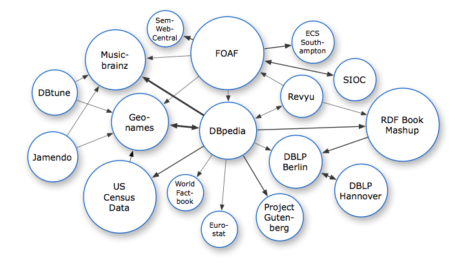
\includegraphics[width=.95\textwidth]{dbpedia_interligacao_dados} 
  \caption{Integração de dados no DBpedia \citep{Auer2007}}
  \label{fig:dbpedia_interligacao_dados} 
\end{figure}

\subsection{Linguagens da Web Semântica}
\label{sec:linguagens_Web_semantica}

De acordo com \citet{Allemang2011}, as tecnologias necessárias para habilitar o novo paradigma da Web já estão disponíveis e envolvem a utilização das linguagens de marcação XML (\emph{Extensible Markup Language}) e HTML (\emph{HyperText Markup Language}), a linguagem RDF (\emph{Resource Description Framework}) para a descrição de ontologias e uma linguagem para consultas em RDF, o SPARQL (\emph{SPARQL query language for RDF}). Em conjunto, essas tecnologias tornam possível a integração de dados provenientes de diferentes bases de dados, documentos, motores de inferência ou qualquer outras fontes de informação que possam expressar conhecimento \citep{Wang}.

\begin{figure}[p]
  \centering
  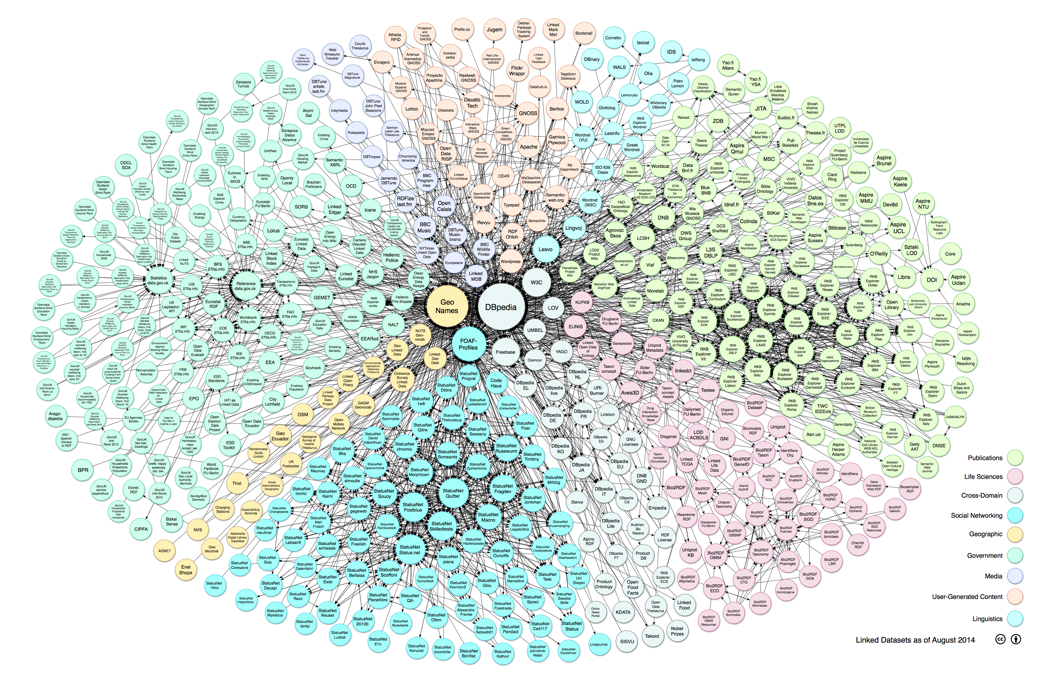
\includegraphics[angle=90, scale=0.65]{lod_graph_agosto_2014} 
  \caption{Integração de fontes de dados abertos em agosto de 2014 \citep{Cyganiak2014}}
  \label{fig:lod_graph_agosto_2014} 
\end{figure}

\subsubsection{HyperText Markup Language (HTML)}
\label{sec:html}

Uma parcela considerável da informação publicada mundialmente na Internet esta disponibilizada através de documentos no formato HTML. Isso ocorre porque essa linguagem foi projetada para estruturar a informação para que um navegador possa interpretar a estrutura dos dados ali definida, e exibi-la de maneira visual para um usuário por meio de botões, textos e outros elementos, que pemitem a um usuário entender e manipular a página com maior facilidade. É baseada em um padrão de marcação de dados estabelecido pela norma ISO8879 que define o SGML (\emph{Standard Generalized Markup Language}) e tem por responsabilidade representar os diversos elementos de uma página, conforme ilustra a Figura~\ref{fig:exemplo_codigo_html}.

\begin{figure}[!ht]
    \begin{lstlisting}[language=HTML,frame=trbl]
<!DOCTYPE html>
<html>
<head>
  <title>Titulo da pagina</title>
</head>
<body>

  <h1>Cabecalho</h1>
  <p>Paragrafo</p>
  
  <!-- comentario -->
  
  <br /> 
  
  <a href="http://www.usp.br">ancora de navegacao (hyperlink)</a>
  
</body>
</html>
    \end{lstlisting}
    \caption{Exemplo de código HTML}
    \label{fig:exemplo_codigo_html} 
\end{figure}

\subsubsection{\emph{eXtended Markup Language} (XML)}
\label{sec:xml}

Em virtude da publicação de informação em larga escala nos meios eletrônicos, tornou-se necessário a existência de um mecanismo capaz de facilitar a troca de uma grande variedade de dados \citep{W3C_XML}. Nesse contexto, o XML surge como solução para este problema, diferentemente do HTML que foi projetado para a marcação de estrutura de exibição em navegadores. Exemplos da versatilidade da aplicação do XML vão desde páginas na Internet, livros, interfaces de programação ou a representação bancos de dados relacionais e seu conteúdo permitindo inclusive o processamento de dados que não estavam previamente armazenados como XML \citep{Wang}. Além disso, a manipulação de um documento XML é feita de maneira trivial pela grande maioria das linguagens de programação \citep{Heath2008},
 
Um documento XML consiste em unidades de armazenamento chamadas de entidades e que formam, em conjunto, uma árvore de nós ordenados. Essas entidades, formadas por caracteres, delimitam os dados através de marcações formando assim o modelo de armazenamento da informação e a estrutura lógica do documento. Além disso, a ordem entre as entidades é relevante, sendo que sua alteração pode inviabilizar a interpretação do documento por ferramentas de software. Dessa maneira, permite-se a criação de rótulos como <cep> ou <nome> , como ilustrado pela Figura~\ref{fig:exemplo_codigo_xml}, que podem ser interpretados a partir da implementação de programas. 

\begin{figure}[!ht]
    \begin{lstlisting}[language=XML]
<?xml version="1.0" encoding="UTF-8"?>
<pessoa>
	<nome>Felipe</nome>
	<sobrenome>Pierin</sobrenome>
	<email>fpierin@ime.usp.br</email>
	<geolocalizacao latitude="-23.558745" longitude="-46.731859" />
	<endereco>
		<cep>05508-090</cep>
		<cidade>Sao Paulo</cidade>
	    <rua>Rua do Matao, 1010</rua>
	</endereco>
</pessoa>	
    \end{lstlisting}
    \caption{Exemplo de um documento XML}
    \label{fig:exemplo_codigo_xml} 
\end{figure}

Um documento XML conciso respeita certas condições simples, como é possível verificar na Figura~\ref{fig:exemplo_codigo_xml}. A primeira condição é que toda marcação tem seu inicio e fim. Isso significa que um rótulo do tipo ``<nome>'' obrigatoriamente tem seu contraponto ``</nome>'' a menos que ele seja auto-contido como o exemplo da ``geolocalizacao'' na linha 6. Além disso o documento está contido em uma única marcação e todas elas estão aninhadas. A linha 7, por exemplo, mostra uma tag ``< endereco>'' que contém outras tags filhas. No entanto, como essas estruturas não possuem semântica sobre o significado, faz-se necessário o entendimento da estrutura por parte do projetista do sistema \citep{Allemang2011}.

\subsubsection{\emph{Resource Description Framework} (RDF)}
\label{sec:rdf}

Na Web Semântica, quando queremos nos referir a algo ou a algum conceitos utilizamos recursos (resources). Desse modo, todas as entidades são definidas como recursos, bem como os seus relacionamentos \citep {Allemang2011}. Nesse sentido, o RDF é uma recomendação da W3C para padronizar o uso de descrições de metadados de recursos baseados na Web \citep{VanDeursen2008} para representar, entre outras coisas, informações pessoais, redes sociais, metadados de artefatos digitais e promover meios de integrar fontes diferentes de informação visando facilitar a troca, fusão e compartilhamento de dados por aplicações diversas. As iniciativas DBPedia, Linked Open Data e o projeto Schema.org auxiliam a transformação dos dados para RDF,  permitindo assim a interligação entre as diversas fontes existentes \citep{Heath2008}.

O RDF é uma extensão do mecanismo de \emph{hyperlinks} e faz a conexão entre recursos da Web atual usando identificadores chamados URI (\emph{Uniform Resource Identifier}) que definem o relacionamento entre as entidades que desejamos descrever. Desse modo, conforme exemplificado pela Figura~\ref{fig:estrutura_triplas_rdf}, a estrutura básica de um documento RDF possui três elementos chaves: o sujeito, um predicado e o objeto de referência. O sujeito ao qual estabeleceremos atributos como, por exemplo, uma pessoa, um automóvel ou uma faculdade, uma entidade objeto que define algum valor tal qual um nome, uma cor ou uma matéria, e um predicado que estabelece a relação entre esse sujeito e a entidade objeto como, por exemplo, ``conhece'', ``é amigo de'', ``é filho de''. No exemplo anterior, é possível observar que o sujeito é ``Felipe Pierin'', representado pelo URI ``\url{http://www.example.org/persons/Felipe_Pierin}'', o predicado é ``mora\_em'' (\url{http://www.example.org/properties/mora_em}) e o objeto ``São Paulo'' (\url{http://www.example.org/places/Sao_Paulo}).

\begin{figure}[!ht]
  \centering
  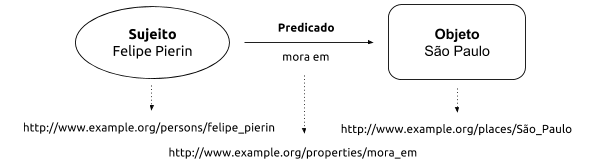
\includegraphics[width=.70\textwidth]{estrutura_triplas_rdf} 
  \caption{Estrutura básica de uma tripla RDF}
  \label{fig:estrutura_triplas_rdf} 
\end{figure}

Ao expandir esse simples modelo para inúmeras conexões, alcançamos uma rede de recursos de informações, inter-relacionados por propriedades que estabelecem relações entre triplas. O resultado disso é um grafo RDF conforme exemplificado pela Figura~\ref{fig:grafo_rdf}. Essa condição é fundamental porque permite que as informações sejam associadas com facilidade e favorece a interpretação por máquinas, uma vez que descreve uma parcela considerável dos dados que são processados por elas. \citep{Allemang2011}. Além disso, como a publicação e conversão de documentos em RDF adiciona semântica ao recursos, ela também promove a integração da informação na Internet proveniente de fontes de dados diversas, uma vez que unifica o entendimento a respeito de um conteúdo, permite um melhor entendimento das máquinas a respeito de um determinado domínio e ainda torna possível a busca de conteúdo relevante por meio de linguagem padrão de consulta, o SPARQL \citep{Heath2008}.

\begin{figure}[!ht]
  \centering
  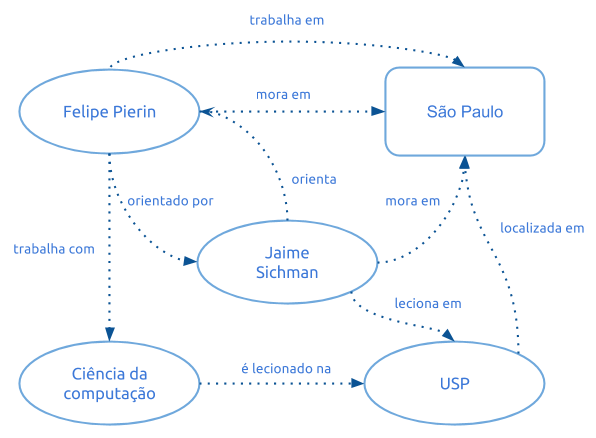
\includegraphics[width=.60\textwidth]{grafo_rdf} 
  \caption{Exemplo de grafo RDF}
  \label{fig:grafo_rdf} 
\end{figure}

Por fim, outra propriedade relevante de um documento RDF é que ele pode ser representado em uma estrutura XML, como ilustrado pela Figura~\ref{fig:exemplo_codigo_rdf}. Nesse exemplo há a definição de um objeto do tipo ``Person'' e que possui um nome definido na marcação ``name'' e um email definido por ``mbox'''. Essa forma de apresentação é denominada RDF/XML e têm sido amplamente utilizada para retratar informações semanticamente anotadas.

\begin{figure}[!ht]
    \begin{lstlisting}[language=XML]
<rdf:RDF xmlns:rdf="http://www.w3.org/1999/02/22-rdf-syntax-ns#"
         xmlns:foaf="http://xmlns.com/foaf/0.1/">
 <foaf:Person>
   <foaf:name>Felipe Pierin</foaf:name>
   <foaf:mbox rdf:resource="fpierin@ime.usp.br"/>
 </foaf:Person>
</rdf:RDF>
    \end{lstlisting}
    \caption{Exemplo de um documento RDF em XML}
    \label{fig:exemplo_codigo_rdf} 
\end{figure}

\subsubsection{\emph{SPARQL Protocol and RDF Query Language} (SPARQL)}
\label{sec:sparql}

Em virtude do documento RDF poder ser entendido como um grafo direcionado para a representação de informação, iniciativas como o SPARQL nasceram para aproveitar essa característica. O protocolo de busca em RDF é, de maneira simplificada, uma linguagem de consulta de correspondência em grafos. Desse modo, levando em consideração uma fonte de dados em RDF, a consulta seria um padrão combinado contra essa fonte e os valores obtidos a partir dessa correspondência são processados para dar a resposta \citep{Perez2006}. Além disso, uma consulta SPARQL não precisa ser restrita a uma única fonte de informação (\emph{endpoint} SPARQL), isso é, vários grafos RDF podem ser combinados dentro de uma única pesquisa, sejam eles documentos RDF nativos ou gerados em tempo de execução via outros sistemas intermediários \citep{W3C_SPARQL}. Por esse motivo, essa linguagem é fundamental no que diz respeito ao Linked Data pois é ela que permite a extração de conhecimento dos diversos endpoints SPARQLs distribuídos \citep{Singh2010}.

Conforme observado por \citet{Perez2006}, uma consulta SPARQL apresenta três partes fundamentais: a correspondência de padrões, os modificadores de resultado e o resultado final. No que diz respeito a correspondência de padrões, a linguagem não só apresenta características de correspondência de padrões em gráficos tais quais partes opcionais, união, aninhamento e filtragem como também permite restringir a qual fonte de dados será aplicada. Já os modificadores de resultado permitem modificar os valores encontrados uma vez que a saída padrão já foi computada. Por fim, o resultado final pode ser tanto um valor específico,  como sim ou não, ou até mesmo um sub-grafo das fontes iniciais utilizadas na consulta. Um exemplo de um código SPARQL é ilustrado na Figura~\ref{fig:exemplo_codigo_sparql}. Na primeira linha o prefixo (PREFIX) ``foaf'' indica que será utilizado para representar a fonte de dados ``http://xmlns.com/foaf/0.1/''. Na segunda linha há uma restrição de informação com o comando ``SELECT'' que possui um filtro ``WHERE'' para recuperar todas as triplas conectadas pela ligação ``foaf:name''.

\begin{figure}[!ht]
    \begin{lstlisting}[language=SPARQL]
PREFIX foaf:  <http://xmlns.com/foaf/0.1/>
SELECT ?name
WHERE {
    ?person foaf:name ?name .
}
    \end{lstlisting}
    \caption{Exemplo de consulta SPARQL}
    \label{fig:exemplo_codigo_sparql} 
\end{figure}

\section{Mineração de dados}
\label{sec:mineracao_dados}

A mineração de dados é uma área de pesquisa que almeja a extração do conhecimento útil existente em uma grande quantidade de dados. Seu foco está concentrado em buscar padrões e regras previamente desconhecidos usando, por exemplo, métodos estatísticos, modelos matemáticos e algoritmos de aprendizado de máquina \citep{Quboa2013, Kabir2014}. Pode ser dividida em três sub-áreas: mineração de dados (\emph{data mining}), mineração de textos (\emph{text mining}) e mineração na Web (\emph{Web mining}). Além disso, pode manipular  dados estruturados ou não estruturados \citep{Singh2010}. Enquanto a mineração de dados lida com dados organizados e estruturados que estão geralmente armazenados em uma base de dados, a mineração de textos, por sua vez, lida com dados não-estruturados. Já a mineração na Web se situa entre os dois extremos, combinando técnicas de ambas para aplicar no vasto repositório de documentos da Internet \citep{Singh2010, Quboa2013}.

De acordo com o trabalho de \citet{Sleiman2011}, a recuperação da informação útil pode ser facilitada por meio de extratores classificados em dois grupos distintos: os baseados em heurística ou em regras. Além disso, regras de extração de informação podem ser supervisionadas, quando há necessidade de treinamento de um algoritmo, ou não-supervisionadas quando essa necessidade inexiste. As regras comuns de extração de informações e reconhecimento de padrões variam de expressões regulares a gramáticas livres de contexto, regras de primeira ordem, tradutores ou modelos baseados em linguagens especificas como XQuery ou XPath. 

O reconhecimento de padrões pode ser feito de modo manual ou a partir de técnicas supervisionadas de aprendizado de máquina que variam desde a extração de palavras chaves usando o método tf.idf, conhecido da área de Recuperação de Informação (Information Retrieval), a técnicas que avaliam as estruturas sintáticas do HTML ou a linguagem natural em consideração, até técnicas que extraem a referência para uma estrutura modelo alvo, como uma ontologia \citep{Stumme2006}. Sistemas como o RAPIER \citep{Califf2004} e o BWI \citep{Freitag2000}, por exemplo, fazem essa tarefa a partir de comparação de padrões em torno da informação relevante com a estrutura geral, calculando a frequência relativa das palavras. Já o modelo de \citet{May} se baseia na estrutura sintática dos documentos analisados usando XPath.

A linguagem XPath foi construída de forma a permitir a recuperação e a manipulação simples de textos, números ou valores booleanos em documentos XML \citep{Clark1999}; entretanto, também pode ser aplicada a outras documentos com estrutura parecida,  como o HTML. Constituída de uma sintaxe compacta, lembra a notação de caminhos em URLs uma vez que é utilizada tendo em foco a localização de um conteúdo na estrutura hierárquica do arquivo alvo. O XPath modela um documento XML como uma árvore de nós, incluindo nós de elemento, nós de atributo e nós de texto. Em resumo, define uma maneira de calcular um valor de sequência de caracteres para cada tipo de nó. Tomando como exemplo a Figura~\ref{fig:exemplo_documento_xml_xpath}, utilizando a expressão XPath ``/universidades/universidade/sigla'', obteremos como resultado a sequência de valores ``USP'', ``Unicamp'', ``UFRJ'' e ``UFSC''.

\begin{figure}[!ht]
    \begin{lstlisting}[language=XML]
<?xml version="1.0" encoding="UTF-8"?>
<universidades>
	<universidade>
	  <nome lang="pt">Universidade de São Paulo</title>
	  <sigla>USP</sigla>
	  <alunos>94875</price>
	</universidade>
	<universidade>
	  <nome lang="pt">Universidade Estadual de Campinas</title>
	  <sigla>Unicamp</sigla>
	  <alunos>40850</price>
	</universidade>
	<universidade>
	  <nome lang="pt">Universidade Federal do Rio de Janeiro</title>
	  <sigla>UFRJ</sigla>
	  <alunos>55887</price>
	</universidade>
	<universidade>
	  <nome lang="pt">Universidade Federal do Santa Catarina</title>
	  <sigla>UFSC</sigla>
	  <alunos>46225</price>
	</universidade>
</universidades>
    \end{lstlisting}
    \caption{Exemplo de documento XML}
    \label{fig:exemplo_documento_xml_xpath} 
\end{figure}

Embora existam diferentes técnicas para a mineração de dados em documentos, todas elas técnicas podem ser encapsuladas de maneira tal que uma requisição para um documento, por exemplo escrito em RDF, possa ser reescrita através de um mediador entre cliente e servidor que irá realizar a tradução da requisição da página, extrair a informação relevante e envia-lá ao cliente \citep{Berendt2004, Kushmerick1997}. Isso permite que elas possam ser reaproveitadas dentro de arquiteturas com contextos específicos que não só a mineração de dados. Neste trabalho, as informações extraídas de portais na Internet são reescritas como triplas RDF.

\subsubsection{Mineração na Web}
\label{sec:mineracao_dados_Web}

A mineração na Web é um processo de extração de informação ou conhecimento usando diferentes técnicas de mineração, como regras de descoberta de associação, agrupamento e classificação aplicadas a fontes de dados expostas na Internet \citep{Zhang2011, Quboa2013}. Conforme \citet{Quboa2013} e \citet{Stumme2006} a área pode ser dividida em três categorias (Figura~\ref{fig:hierarquia_mineracao_Web}): a mineração de uso na Web, a mineração de estrutura na Web e a mineração de conteúdo na Web. A primeira busca entender o comportamento de um determinado usuário na Internet valendo-se dos registros deixados por ele em arquivos de logs como o do navegador Web. Com isso, essa categoria de pesquisa visa criar ou melhorar serviços, tornando-os mais personalizados. A segunda é uma técnica que tenta reconhecer informações de topologia entre fontes de informações na Internet. Já a mineração de conteúdo atem-se à mineração de informação em textos e imagens a fim de auxiliar uma pessoa a encontrar resultados mais precisos conforme o seu interesse.

\begin{figure}[!ht]
  \centering
  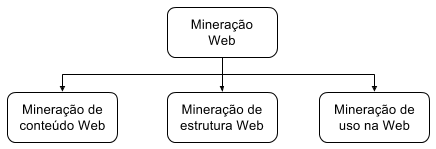
\includegraphics[width=.70\textwidth]{hierarquia_mineracao_web_simplificado} 
  \caption{Categorias da Mineração Web}
\end{figure}
  \label{fig:hierarquia_mineracao_Web} 

A mineração de conteúdo é um processo que aproveita a natureza da maioria dos documentos semi-estruturados contidos na Web a partir da exploração de anotações HTML e de suas marcações XML \citep{Stumme2006}. Isso ocorre porque essas fontes de dados carregam não só a informação de como uma determinada página na Web deve ser apresentada para um usuário no navegador mas também a estrutura lógica de como esses dados são apresentados. Dessa maneira, ao identificar os padrões de como um determinado texto ocorre em um recurso Web, é possível elaborar processos automatizados para extrair o conteúdo relevante e então mapeá-los para uma nova estrutura que permita um melhor gerenciamento do domínio da informação. Em geral, as técnicas de extração de informação visando à construção da Web semântica dependem muito do reconhecimento da informação em documentos que geralmente é feita a partir da descoberta de padrões \citep{Berendt2004}.

De acordo com \citet{Zhang2011}, a mineração de dados na Web é alcançada por meio de quatro passos conforme ilustra a Figura~\ref{fig:processo_Web_mining}: (i) a descoberta de recursos que compreende a escolha e obtenção de dados de um recurso na Web seja ele um documento eletrônico, um e-mail ou registros de navegação de um usuário; (ii) a escolha da informação e o pré-processamento que envolve remover os dados irrelevantes à informação escolhida; (iii) a busca automatizada do padrão por meio de ferramentas de mineração como, por exemplo, o XPath e (iv) a análise do padrão encontrado, que envolve a validação por meios automatizados ou a partir da avaliação humana.

\begin{figure}[!ht]
  \centering
  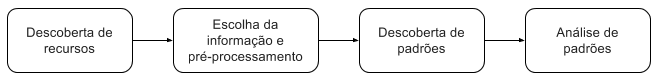
\includegraphics[width=.90\textwidth]{processo_web_mining} 
  \caption{Processo de Web Mining \citep{Zhang2011}}
  \label{fig:processo_Web_mining} 
\end{figure}

\subsubsection{Mineração de dados para a Web Semântica}
\label{sec:mineracao_Web_semantica}

Embora a mineração Web forneça meios para extrair conhecimento relevante na Web, a maioria dos dados espalhados na rede é desestruturada, a ponto de tornar complicada a agregação de conteúdos sob uma estrutura comum \citep{Kabir2014}. Nesse contexto, a Web Semântica pode ser combinada com essas técnicas de mineração na Web formando uma área de pesquisa que engloba as áreas de Mineração de dados e Web Semântica para suprir essa deficiência.

A mineração de dados voltada para a Web semântica (\emph{Semantic Web Mining}) combina o desafio de fazer com que dados sejam compreensíveis para máquinas com o de extrair conhecimento útil escondido nesses documentos de forma automática por meio de técnicas de mineração em dados \citep{Stumme2006}. Esse modo de recuperação de informação é válido tanto em cenários bem estruturados, como tabelas em banco de dados, em textos semi-estruturados, ou até naqueles textos sem estrutura alguma, de maneira que podem ser aplicados para ajudar a criar a Web Semântica.

\section{Integração de dados}
\label{sec:integracao}

Vivemos em meio a um cenário em que a informação é constantemente exposta não só pelos meios tradicionais da Web, a partir de páginas dinâmicas HTML, mas também facilitada nos diversos aplicativos por meio de interfaces para a recuperação de informação em software chamadas API (\emph{Application Programming Interface}), cujo  propósito é o de permitir ao usuário final a criação de sistemas mais ricos que integram o conteúdo do aplicativo com outros de seu interesse. Exemplos de empresas que trabalham dessa forma são os mais diversos e compreendem grandes empresas de tecnologia como Facebook, LinkdIn, Amazon, Youtube, Dropbox, Instagram, Flickr, Twitter, entre outros. Por outro lado, toda essa informação e uma considerável parcela do conteúdo da Internet está confinado a esses silos de informação e isso dificulta uma visão homogênea e extração de dados sobre um determinado domínio de interesse \citep{Heath2008, Civili2013}. 

A necessidade em gerenciar vastas quantidades de informações provenientes de fontes de dados heterogêneas têm incentivado a pesquisa em maneiras mais inteligentes de se realizar a integração de dados sobre um mesmo domínio \citep{Wang, Vettor2014}.
A integração e busca em fontes de dados heterogêneas tem sido um tópico muito explorado uma vez que é cada vez mais complicado o acesso a informações relevantes nesse contexto dada a velocidade de exposição de novos conteúdos e a grande quantidade de diferentes tipos de formatos. São dados em grande quantidade, desorganizados e desconectados. Desse modo, o objetivo da integração de dados é prover ao usuário uma maneira de acesso uniforme a múltiplas fontes de dados heterogêneas \citep{Wang}. Entretanto, ainda são poucas as soluções genéricas para converter e conectar fontes de dados de origens diversas em um conjunto de dados único e coerente mas todas elas podem ser categorizadas em um modelo de integração no qual todos os dados são recuperados e agrupados dentro de um mesmo banco de dados ou em um modelo que se vale de um processo bem definido para a integração de informação mas que não depende de um banco de dados centralizado.

A integração de dados pode ser alcançada por meio de uma dentre duas estratégias distintas conhecidas como Global As View (GAV) ou Local As View (LAV) \citep{Abdellaoui2015, Wang2017, Putra2017}. A estratégia GAV é tradicionalmente utilizada para aplicações em que há consultas federadas nas quais uma única consulta dispara pesquisas em múltiplas fontes de dados e unifica a informação recuperada por meio de múltiplas camadas de abstrações. Já o método LAV realiza a materialização desses dados em um banco de dados único. Contudo, cada uma dessas técnicas possuem vantagens e desvantagens. O método GAV, por exemplo, pode não ser aplicável em situações em que existam fontes de dados faltando para a visão completa de um determinado domínio como, por exemplo, um portal estiver fora do ar e passar por modificações nos dados dele. Por outro lado não depende de materialização dos dados em um banco centralizado o que pode ser um estimulo do ponto de vista financeiro\citep{Putra2017}. A estratégia LAV, por sua vez, trabalha melhor em fontes de dados incompletas ou que não possam ser acessadas em um determinado momento, como no contexto da Internet \citep{Putra2017}, ou em situações nas quais a realização de uma consulta Federada seja lenta demais para trazer um resultado dentro de um tempo aceitável. A fim de evitar problemas com fontes de dados incompletas, portais inacessíveis ou lentidão para consultas federadas, neste trabalhou adotou-se uma abordagem LAV.

A combinação de dados não é um processo trivial e exige soluções que vão desde formas para lidar com as divergências entre documentos, duplicações e ruídos. É um processo que exige adaptação das fontes de informação a nível sintático, estrutural e semântico \citep{Vettor2014}. A necessidade de atuar no nível sintático é justificada porque o formato dos dados pode ser diferente já que podemos, por exemplo, querer combinar a informação contida em um banco de dados com outra contida em documentos XML. Mesmo que os documentos sejam do mesmo tipo, por exemplo páginas HTML, a estrutura pode não ser igual, e portanto deve-se atuar no nível estrutural. Por fim, é necessário atuar no nível semântico porque a representação do conhecimento nos documentos que terão a informação combinada pode ser diferente. Além disso, ao recuperar e combinar informações provenientes de múltiplos recursos é possível que exista repetição de informação, ruídos, imprecisão ou outros tipos de inconsistência que podem causar perda de significado ou mal-entendidos, que são prejudiciais ao resultado final da integração \citep{Vettor2014}.

\section{Trabalhos relacionados}
\label{sec:trabalhos_relacionados}

A fim de auxiliar a resolução de possíveis problemas decorrentes da integração de dados, máquinas podem ser empregadas para desempenhar um papel relevante. Em outras palavras, há a necessidade de oferecer algoritmos e descrições semânticas precisas dos dados trabalhados para que o computador possa interpreta-las corretamente e entregar melhores resultados \citep{Vettor2014}. Por esse motivo, vários linhas de estudos convergem e vão desde o uso de ontologias para mapear um domínio comum visando a solução do problema da integração de dados heterogêneos \citep{Ahmed2008}, a integração baseada em Sistemas Multi-Agentes \citep{Sui2009} ou o acesso a informação baseado em ontologias \citep{Civili2013, Lembo2014, Kharlamov2013}.  

Levando em consideração que a maior parte dos documentos existentes na Web está definida valendo-se de formatos semi-estruturados, e.g. XML, é de se esperar que a integração de dados seja feita por meio de anotações semânticas \citep{May}. Por essa razão, iniciativas como o SIOC \citep{Bojars2008} buscam uma proposta valendo-se do apontamento ontológico em Resource Description Framework (RDF) \citep{RDFWorkingGroup2014} mas visando à conexão de informação proveniente de comunidades sociais tais como Flickr, Youtube, Facebook e Wikipédia por meio do mapeamento das APIs disponibilizadas por estes sites. Já trabalhos como o de \citet{Cardoso2006} buscam criar uma ontologia para o a industria do turismo. 

Utilizar o conteúdo já existente na Web atual e convertê-lo para a Web semântica é outra linha de pesquisa. Ela visa à integração de informação, a reutilização de dados e a evolução da Web atual para a Web semântica. O Deep Annotation, por exemplo, é um framework para prover anotação para um vasto conjunto de dados a partir de uma ferramenta que é simples e intuitiva \citep{Handschuh2003}. Trabalhos como o de \citet{AndreasHess} buscam este objetivo por meio de um mapeamento ontológico da informação a partir de um mecanismo semi-automático de marcação, no qual os usuários escolhem ``tags'' dentre uma lista de sugestões. Outros trabalhos como o de \citet{May} fazem o uso da linguagem de consulta XPath\footnote{\url{https://www.w3.org/TR/xpath-31/}} para selecionar os nós de um documento XML, encontrar estruturas relevantes do documento para então mapeá-las ontologicamente. Já trabalhos como o Bottari \citep{Balduini2012} aliam a interpretação da diversidade de conteúdo produzido das publicações de pessoas no Twitter, seguida de mapeamento semântico desses dados em uma ontologia padronizada. A partir disso aplica o resultado obtido a fim de proporcionar uma realidade aumentada capaz de sugerir pontos de interesse como restaurantes.

A orquestração de serviços disponibilizados na Internet é outra abordagem de estudo amplamente explorada por pesquisadores. Trabalhos como o SBWS\footnote{\url{http://asio.bbn.com/sbws.html}} e o ASSAM \citep{Hess2003, Hess2004} buscam realizar mapeamento semântico sobre uma descrição de serviços WSDL\footnote{\url{https://www.w3.org/TR/wsdl}} que funcionam sobre o procolo SOAP\footnote{\url{https://www.w3.org/TR/soap/}}. Com isso, um usuário pode anotar de forma semântica um WebService a partir de sugestões de classes ontológicas para marcar cada elemento da descrição do serviço exposto. O projeto Satine\footnote{Dogac2004} é outro exemplo. Ele busca promover a criação e desenvolvimento de serviços Web enriquecidos semanticamente mas visando a integração de informação no domínio de viagens de maneira a padronizar e simplificar o processo de busca de passagens aéreas e hospedagem no domínio de viagens.

Outros estudos buscam mapear serviços REST\footnote{\url{https://www.w3.org/2001/sw/wiki/REST}} em RDF de maneira a permitir a busca de conteúdo através de consultas SPARQL \citep{Battle2008}. Isso porque ao publicá-los em RDF, os dados ficam acessíveis via uma linguagem de pesquisa padrão \citep{W3C_SPARQL} e isto torna mais fácil a integração de diferentes fontes, uma vez que os dados passam a ser entendidos por máquinas\citep{Heath2008}. Já trabalhos como o SOARI \citep{Nardin2011} buscam tornar possível a interoperabilidade entre sistemas heterogêneos e distribuídos por meio de uma ontologia comum a partir da qual podem trocar informação com um mesmo entendimento de significado. 

A exposição de dados ocultos é outro grande problema relacionado à integração da informação na Internet. Ao passo em que é cada vez maior o número de aplicações fazendo o uso de bancos de dados relacionais, o mapeamento semântico pode ser considerado como um instrumento para a relação e extração de informação relevante a partir de diferentes fontes de dados, tornando mais clara a importância em revelar dados relacionais como RDF ou Linked-Data \citep{Hellmann2009}. Ferramentas já conhecidas como o VirtuosoRDF\footnote{\url{http://virtuoso.openlinksw.com/}}, D2RQ\footnote{\url{http://d2rq.org/}}, entre outras, estão aptas para uso com a capacidade de gerar representações RDF que derivam diretamente de acordos implícitos e explícitos dos bancos de dados (BD) relacionais \citep{Hellmann2009}, permitindo assim o acesso à informação baseado em ontologias.

O paradigma para a integração de dados provenientes de fontes distintas é o OBDA (\emph{Ontology-based data access}), que baseia o acesso à informação por meio de ontologias sobre um mesmo domínio de conhecimento de interesse \citep{Civili2013, Lembo2014, Bienvenu2013}. Essa capacidade se dá a partir de uma arquitetura de três níveis constituída pela ontologia,  fontes de dados e  mapeamento entre ambas \citep{Lembo2014, Civili2013}. Dessa forma é possível extrair informações de uma fonte de dados a partir de consultas que usam ontologias \citep{Bienvenu2013}. Nesse contexto, um dos primeiros representantes desse modelo é o D2RQ \citep{Calvanese2016} que realiza o mapeamento do banco de dados em estruturas semanticamente anotadas que permitem o acesso à informação por meio dessas ontologias.

O OBDA pode ser usado para enriquecer o conhecimento em uma fonte de dados incompleta a ponto de trazer um conjunto mais completo de respostas para uma consulta aproveitando as capacidades de inferências por meio do raciocínio lógico dos bancos de dados semânticos \citep{Bienvenu2013, Calvanese2016}. Suponha uma fonte de dados que descreva um paciente com um Linfoma e outro paciente com Melanoma. Uma pesquisa sobre essa base de dados apenas de posse apenas dessas informações impede que seja pesquisado de forma satisfatória todos os pacientes que possuem algum tipo de câncer. Por outro lado, podemos enriquecer esses dados a partir do uso de ontologias que classificam ambos como tipos de câncer. Agora é possível extrair um resultado com um conjunto mais completo de informações úteis para um hospital ou um médico.

Sistemas como o Ontop \citep{RodriguezMuro2013OntopAW, Calvanese2016} e o o MastroStudio \citep{Civili2013} são exemplos de implementações ODBA e que expõem bancos de dados relacionais como grafos RDF virtuais a partir de mapeamentos entre ontologias e o banco de dados. O grafo RDF pode ser então ser consultado usando SPARQL, já que o sistema traduz a consulta para a linguagem SQL de maneira transparente ao usuário, de maneira tal que ele não precisa ter conhecimento sobre os bancos de dados nem sobre o relacionamento entre eles.

\section{Síntese}

A proposta de integração de informação dos portais na Web almejada neste trabalho utiliza tecnologias apresentadas neste capítulo e envolve técnicas de recuperação de dados e mapeamento semântico para a integração dos dados espalhados na Web. Ao passo em que as fontes de conteúdo são escolhidas, a recuperação da informação nesses portais acontece por meio de rotinas de extração de dados que, por sua vez, são desenvolvidas manualmente e baseadas na anáĺise dos padrões de repetição dos assuntos relacionados ao domínio escolhido. Desse modo, informações como o nome, endereço ou outros dados relacionados a um determinado evento ou restaurante são recuperadas de maneira automatizada de acordo com regras pré-estabelecidas por meio de expressões capazes de interpretar a estrutura sintática do documento HTML dos diferentes portais e recuperar conteúdo relevante.

O processo de análise da estrutura dos documentos HTML expostos pelos diferentes portais escolhidos em busca de padrões de repetição de informação é realizado manualmente. A interpretação das fontes de dados escolhidas, bem como a transferência da inteligência para a expressão regular, são de responsabilidade do individuo que aplica o modelo proposto neste trabalho. Isso também se aplica no que diz respeito a transferência da informação obtida através da recuperação dos dados aplicada em uma ontologia de maneira a obter dados anotados semanticamente.

Uma vez que os dados são obtidos, uma camada de informação semântica é adicionada utilizando as ontologias descritas no portal Schema.org. Nesse momento, a informação está descrita como triplas RDF que são armazenadas em um banco de dados semântico. As triplas, ao serem persistidas no banco de dados, se integram com os dados que foram obtidos de diferentes portais da Web e são enriquecidas a partir do processo realizado pelo motor de inferência. Nesse momento, o acesso à informação por meio de ontologias pode ser realizado utilizando a linguagem de consulta SPARQL. A informação de diferentes fontes de dados pode então ser recuperada sobre um ponto de vista amplo e centralizado.

No capítulo a seguir, a proposta da arquitetura para integração de dados de portais na Web que utiliza tais tecnologias é detalhada.





